\documentclass[12pt]{article}


%--------- Packages ----------------

\usepackage{wrapfig}
\usepackage{graphicx} % Required for inserting images
\usepackage{tabularx}
\usepackage[a4paper,left=1in,right=1in,top=1in,bottom=1in]{geometry}
\usepackage{enumitem}
\usepackage{newtxtext} % If you need to use Time New Roman
\usepackage{newtxmath} % If you need to use Time New Roman
\usepackage[style=ieee,backend=biber]{biblatex}
\usepackage[british]{babel}
\usepackage{csquotes}
\usepackage{bookmark}
\usepackage{setspace}
\usepackage{fancyhdr}
\usepackage[font=footnotesize,justification=centering]{caption}
\usepackage{hyperref}
\usepackage{float}
\usepackage{caption}   % For controlling captions
\usepackage{setspace}
\usepackage{booktabs}
\usepackage{array}
\usepackage{gensymb}
\usepackage{mathastext}  % Use New Century Schoolbook font for 
\usepackage{textcomp}
\usepackage[upgreek, LGRgreek]{mathastext}


%--------- Set Up ------------------
\setstretch{1.4}
\pagestyle{fancy}
\fancypagestyle{plain}{%
  \renewcommand{\headrulewidth}{0pt}%
  \fancyhf{}}
\addbibresource{references.bib}


% Stuff about lists
\setlist[itemize,1]{itemsep=-0.7em,topsep=0.1pt, before=\vspace{0.5em}}  % Reduce space between items in the first-level list
\setlist[itemize,2]{itemsep=-0.2em,topsep=0pt, parsep=0pt, partopsep=0pt, before=\vspace{-0.6em},after=\vspace{0.6em}}  % Reduce space between items in the second-level list
% Reduce line spacing for second-level lists
\newenvironment{tightitemize}{%
    \begin{itemize}
    \setstretch{1}  % Adjust the number to reduce line spacing
}{%
    \end{itemize}
}

% --- title insert (check title.tex for more)----------

\title{T1 – Heat Engine / Gas Law Apparatus} % TITLE HERE 


%-------- Document -----------------

\begin{document}

\begin{titlepage}


\newcommand{\HRule}{\rule{\linewidth}{0.5mm}} % Defines a new command for the horizontal lines, change thickness here

% ----- Logo UM ---------

\center

\includegraphics[width=15
cm]{Graphics/logoUM.png}\\[1cm]


\textsc{\large PRA3002 Lab Report II}\\

\makeatletter
\rule{\linewidth}{0.2 mm} \\[0.4 cm]
{\huge\bfseries \@title \par} \
\rule{\linewidth}{0.2 mm} \\[1.0 cm]
 \textsc{ Maastricht Science Programme\\2024-2025}\\[1.5cm] % Name of your program

\begin{minipage}{1\textwidth}
\begin{center}
\emph{Author:}\\
Nils Thiessen
\end{center}
\end{minipage}

\begin{minipage}{1\textwidth}\
\begin{center}
\emph{Team members:}\\
Grzegorz Ratajski, Nils Thiessen
\end{center}
\end{minipage}

\vspace{1cm}
\emph{Instructors:}\\
Chris Pawley, Sanne Aarts\\
\vspace{1cm}
\makeatother
{\large 22nd November 2024}\\[2cm] % Date, change the \today to a set date if you want to be precise
\vfill % Fill the rest of the page with whitespace





\end{titlepage}




\fancyhf{}
\setlength{\headheight}{33pt}
\fancyhead[L]{\nouppercase{\leftmark}}
\fancyhead[R]{
\includegraphics[width=0.7cm]{Graphics/UM_SMALL.png}}
\fancyfoot[L]{\emph{PRA3002 Lab Report T1} }
%\pagenumbering{gobble}

%\setmathfont{Cambria Math}  % Set the math font to Cambria 
\addtocounter{page}{1}

\newpage
\fancyhead[L]{\textbf{Contents}}
\tableofcontents
\newpage
%\pagenumbering{arabic} %ensures that pagenumbering starts after table of contents

\fancyhf{}
\setlength{\headheight}{33pt}
\fancyhead[L]{\nouppercase{\leftmark}}
\fancyhead[R]{
\includegraphics[width=0.7cm]{Graphics/UM_SMALL.png}}
\fancyfoot[R]{ \bf\thepage\ \rm }
\fancyfoot[L]{\emph{Lab Report II} }

\newpage
\section{Introduction}
\label{Introduction}

The observations conducted in the lab session centered around observing thermodynamic processes inside a metal cylinder, verifying its properties as an ideal gas and determining work and heat involved when undergoing an Ericsson cycle. Furthermore, the engine's efficiency will be compared to that of the Carnot cycle.  

The explicit notion of viewing heat and work as two closely related energy quantities is rather novel compared to the long history in which the practical implications were already utilized. The first steam engine, although severely lacking in its efficiency, had already been implemented in Britain as early as 1698, and optimized by Newcomen and Watt in the subsequent century \cite{Saslow2020AHO}. Later, the rate of development sped up during the peak of the industrial revolution, where efforts were aimed at improving the efficiency of existing engines \cite{LumenLearning}. In 1824, Sadi Carnot proposed in 1824 the Carnot Cycle as a reversible heat engine, consisting of two isothermal and two adiabatic processes, while also introducing the idea of separate hot and cold reservoirs in which the engines would operate. \cite{Saslow2020AHO}

These achievements were based on a complex history of discoveries, and continued to be. Independently, several scientists reached the conclusion that the internal energy of an isolated system has to stay constant, but can vary in its form, later regarded as the First Law of Thermodynamics. Entropy, its property as a state function and its change under reversible and irreversible processes were outlined in 1865 by Rudolf Claudius \cite{Saslow2020AHO}. These concepts and numerous others lay the foundations of thermodynamics, which can be classified as the study of macroscopic properties of a system, as a result of its molecular behaviour. \cite{LabManual}

\subsection{Theory}
\label{Theory}

The experimental setup includes a metal can which is later connected to a piston tube expanding under higher pressure. By preparing separate heat reservoirs, one can simulate a cycle which the gas undergoes. More precisely, if the gas can be thought of as an ideal gas, the cycle will consist of two isobaric and two adiabatic processes. In between, heat is converted into mechanical work, and it is therefore fundamental to understand the principles behind ideal gasses and thermodynamic processes.

\subsubsection{Ideal Gas Law}
\label{Ideal Gas Law}

In thermodynamics, the key characteristics of a gas system considered in calculation are the pressure $\mathit{P}$, volume $\mathit{V}$, temperature $\mathit{T}$ and the amount of it. The latter is often represented in the number of moles of gas $\mathit{n}$, which equates to $\mathit{N_A = 6.022 \cdot 10^{23}}$ individual molecules. These can be used to define define properties such as internal energy $\mathit{E_{int}}$ or work $\mathit{W}$ for specific situations. By holding certain parameters constant, a number of underlying laws for ideal gasses have been discovered. The assumption of ideal gasses implied an assembly of non-interacting, similar point-like particles performing elastic collisions. Macroscopically, this is a decent approximation for most real processes \cite[pp.~391-395]{Brown}. 

\textbf{Boyle's Law} states that under constant $\mathit{n}$ and $\mathit{T}$, the system's volume is inversely proportional to the pressure: 

\begin{equation}
\label{eq:Boyle's Law}
    \mathit{V \alpha \frac{1}{P}}
\end{equation}

Stated in \textbf{Charles' law}, at constant $\mathit{n}$ and $\mathit{P}$, volume is proportional to the temperature: 

\begin{equation}
\label{eq:Charles' Law}
    \mathit{V \alpha T}
\end{equation}

Note that the absolute temperature scale is is generally applied in thermodynamics, with $\mathit{T}$ measured in Kelvin [K]. Similarly, \textbf{Gay-Lussac's law} related pressure to temperature, under the condition that $\mathit{n}$ and $\mathit{V}$ are held constant. It can already be implied from the previous laws: \cite[pp.~387-391]{Brown}

\begin{equation}
\label{eq:Gay-Lussac's Law}
    \mathit{P \alpha T}
\end{equation}

Lastly, \textbf{Avogadro's law} shows that at constant $\mathit{T}$ and $\mathit{P}$, volume is proportional to the number of moles contained in it: \cite[pp.~387-391]{Brown}

\begin{equation}
\label{eq:Avogadro's Law}
    \mathit{V \alpha n} 
\end{equation}

% https://chem.libretexts.org/Bookshelves/General_Chemistry/Map%3A_Chemistry_-_The_Central_Science_(Brown_et_al.)/10%3A_Gases/10.03%3A_The_Gas_Laws


Combining the relations and introducing a new constant factor $\mathit{R} = 8.314 \frac{J}{Kmol}$, the gas constant, the \textbf{ideal gas law} appears as a result, as seen in Equation \ref{eq:Ideal_Gas_Law}. As the name suggests, the relation holds true for ideal gases. \cite[pp.~391-395]{Brown}

\begin{equation}
\label{eq:Ideal_Gas_Law}
    \mathit{PV = nRT}
\end{equation}

At higher pressures and temperatures, a bigger deviation from ideality occurs for the gas. Hence, a compressibility factor $\mathit{z}$ is introduced in modern analysis. \cite{AHMED201029}

\subsubsection{Work and Heat}
\label{Work-Heat}

Work is done by application of a force $\mathit{F}$ over a distance $\mathit{dx}$. A gas contained in a tube pushing against a piston would exert a force relative to the pressure and the piston's area. If that force causes a change in volume $\mathit{dV}$, the work applied or exerted on the gas is given by: \cite{Ling2016-bs}

\begin{equation}
\label{eq:Work}
    \mathit{dW = PdV}
\end{equation}

For processes between conditions 1 and 2, one can further modify the equation:

\begin{equation}
\label{eq:Work_Int}
    \mathit{W = \int_{V_1}^{V_2} PdV}
\end{equation}

Work is a path-dependent function, the way chosen to get from A to B has an impact on the resultant work. 

\begin{wrapfigure}{r}{0.4\textwidth}  % 'r' for right, and width of 0.4 of the text width
    \centering
    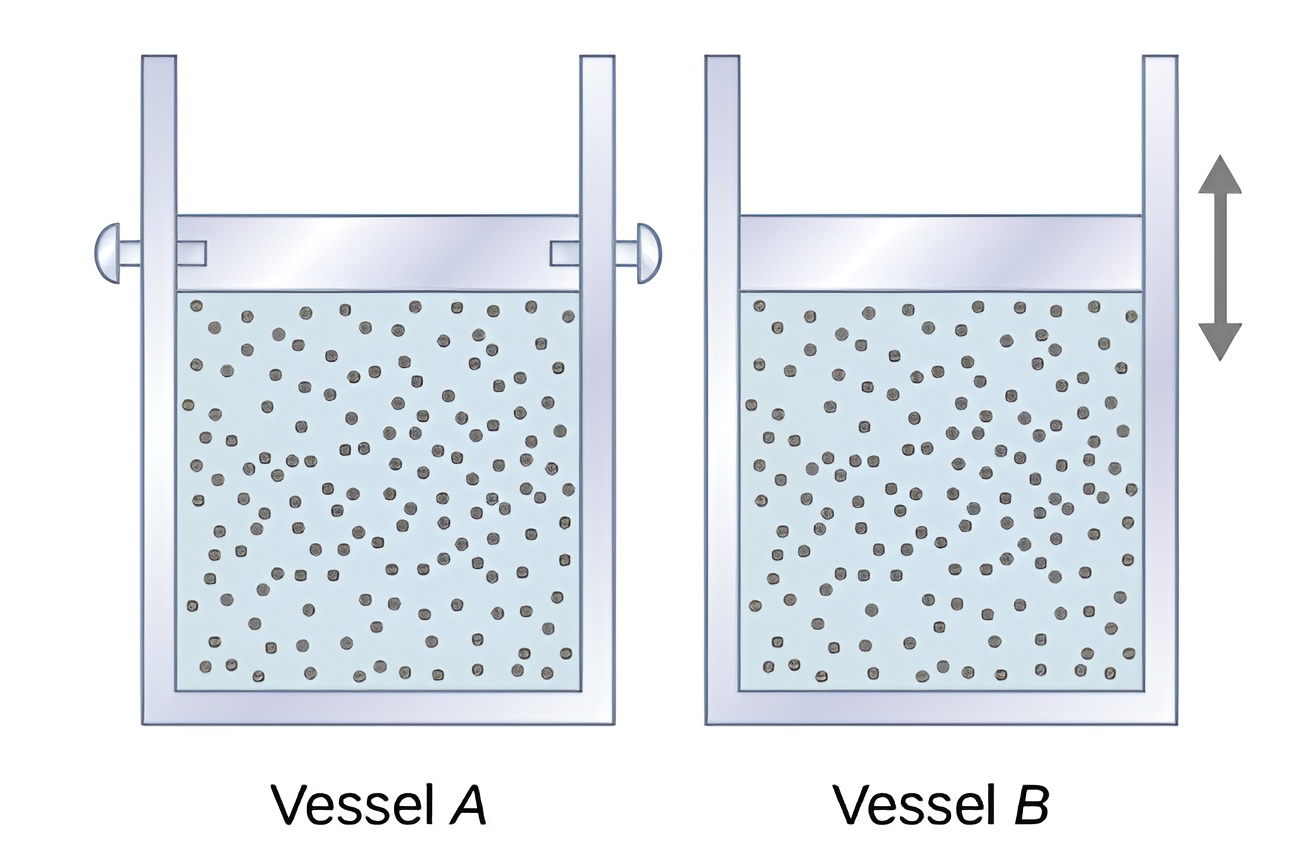
\includegraphics[width=0.4\textwidth]{Graphics/Constant_Diagrams.png}  % Adjust the width of the image
    \caption{Same thermodynamic system, with particles trapped inside a cylinder with a movable piston. Left: Volume is fixed. Right: Pressure is fixed. \cite{Ling2016-bs}  }
    \label{fig:Constants}
\end{wrapfigure}

The other relevant type of energy exchange can be classified as that of heat $\mathit{Q}$. Heat describes the transfer of energy into or out of the system, where $\mathit{Q}$ is negative or positive depending on the convention in which direction heat flow is described \cite{Ling2016-bs}. The amount of heat that is expelled is based on the change in temperature of the system, but also dependent on the number of atoms per molecule, which decides the degrees of freedom of movement. The relationship can be summarized in Equation \ref{eq:Heat}. \cite{Zohuri2019}

\begin{equation}
\label{eq:Heat}
    \mathit{Q = mc \Delta T}
\end{equation}

where $\mathit{m}$ represents mass and $\mathit{c}$ is the heat specific heat. 

The equation can be simplified under specific constraints, which is visualized in Figure \ref{fig:Constants}. If one would fix the piston such that the volume stays the same, the heat related to an infinitesimally small temperature change is given by Equation \ref{eq:C_V}. \cite{Zohuri2019}

\begin{equation}
\label{eq:C_V}
    \mathit{dQ = n C_V dT}
\end{equation}

At constant pressure, Equation \ref{eq:Heat} becomes. 

\begin{equation}
\label{eq:C_P}
    \mathit{dQ = n C_P dT}
\end{equation}

A thermodynamic system contains an internal energy $\mathit{U}$. The total heat exchanged and work done by the system are related in the First Law of Thermodynamics: 

\begin{equation}
\label{eq:1st Law}
    \mathit{\Delta U = Q - W}
\end{equation}

For any process between two equilibrium states, the law should be applicable. \cite{Ling2016-bs}


\subsubsection{Heat Engines and Thermodynamic Processes}
\label{Heat Engines}

\begin{wrapfigure}{r}{0.35\textwidth}  % 'r' for right, and width of 0.4 of the text width
    \centering
    \vspace{-0.75cm}
    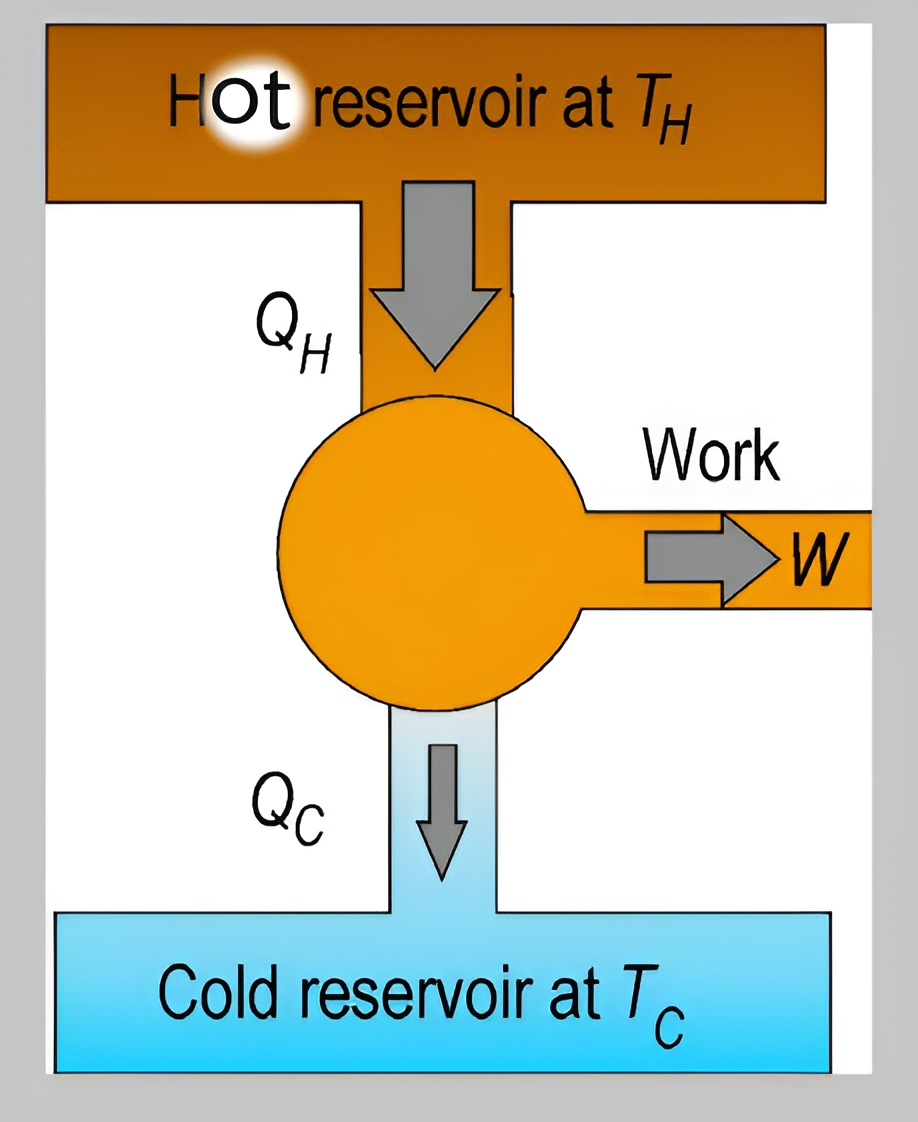
\includegraphics[width=0.35\textwidth]{Graphics/Heat_Engine.png}  % Adjust the width of the image
    \caption{PV-Diagram of the Carnot Cycle. \cite{Bassie2012-pw}}
    \label{fig:Carnot Cycle}
\end{wrapfigure}

In thermodynamics, one usually refers to a system as the part of the universe for which the observations are taken. One is especially interested in the changes in states when interactions with the environment occur. If non-quasi-static, only the beginning and ending state during these thermodynamic processes can be described at thermal equilibrium. In theory, one could slow down the transition to a point where the system appear to always be in thermal equilibrium. \cite{Ling2016-bs}

Heat engines are designed to extract heat and, by cycling through specific types of thermodynamic processes, translate it into work and arrive at the same thermal equilibrium state. The efficiency of each cycle for a given machine is defined by Equation \ref{eq:Efficiency}.

\begin{equation}
\label{eq:Efficiency}
    \mathit{\nu = \frac{W}{Q_h} = 1 - \frac{Q_c}{Q_h}}
\end{equation}

Key to the cyclic nature is a setup consisting of one high-temperature and one cold-temperature reservoir. In the equation, $\mathit{Q_h}$ represents the heat withdrawn from the hot reservoir, $\mathit{W}$ the work delivered and $\mathit{Q_c}$ the heat disposed in the cold reservoir during each cycle. 

The Carnot Cycle is the ideal model for a heat engine. Consisting of two adiabatic and two isothermal processes, it is the cycle with the maximum possible efficiency. The steps are visualized in Figure \ref{fig:Carnot Cycle}, where the area enclosed by the graphs is the net work of the heat engine.

\begin{figure}[H] % 'r' for right, and width of 0.4 of the text width
    \centering
    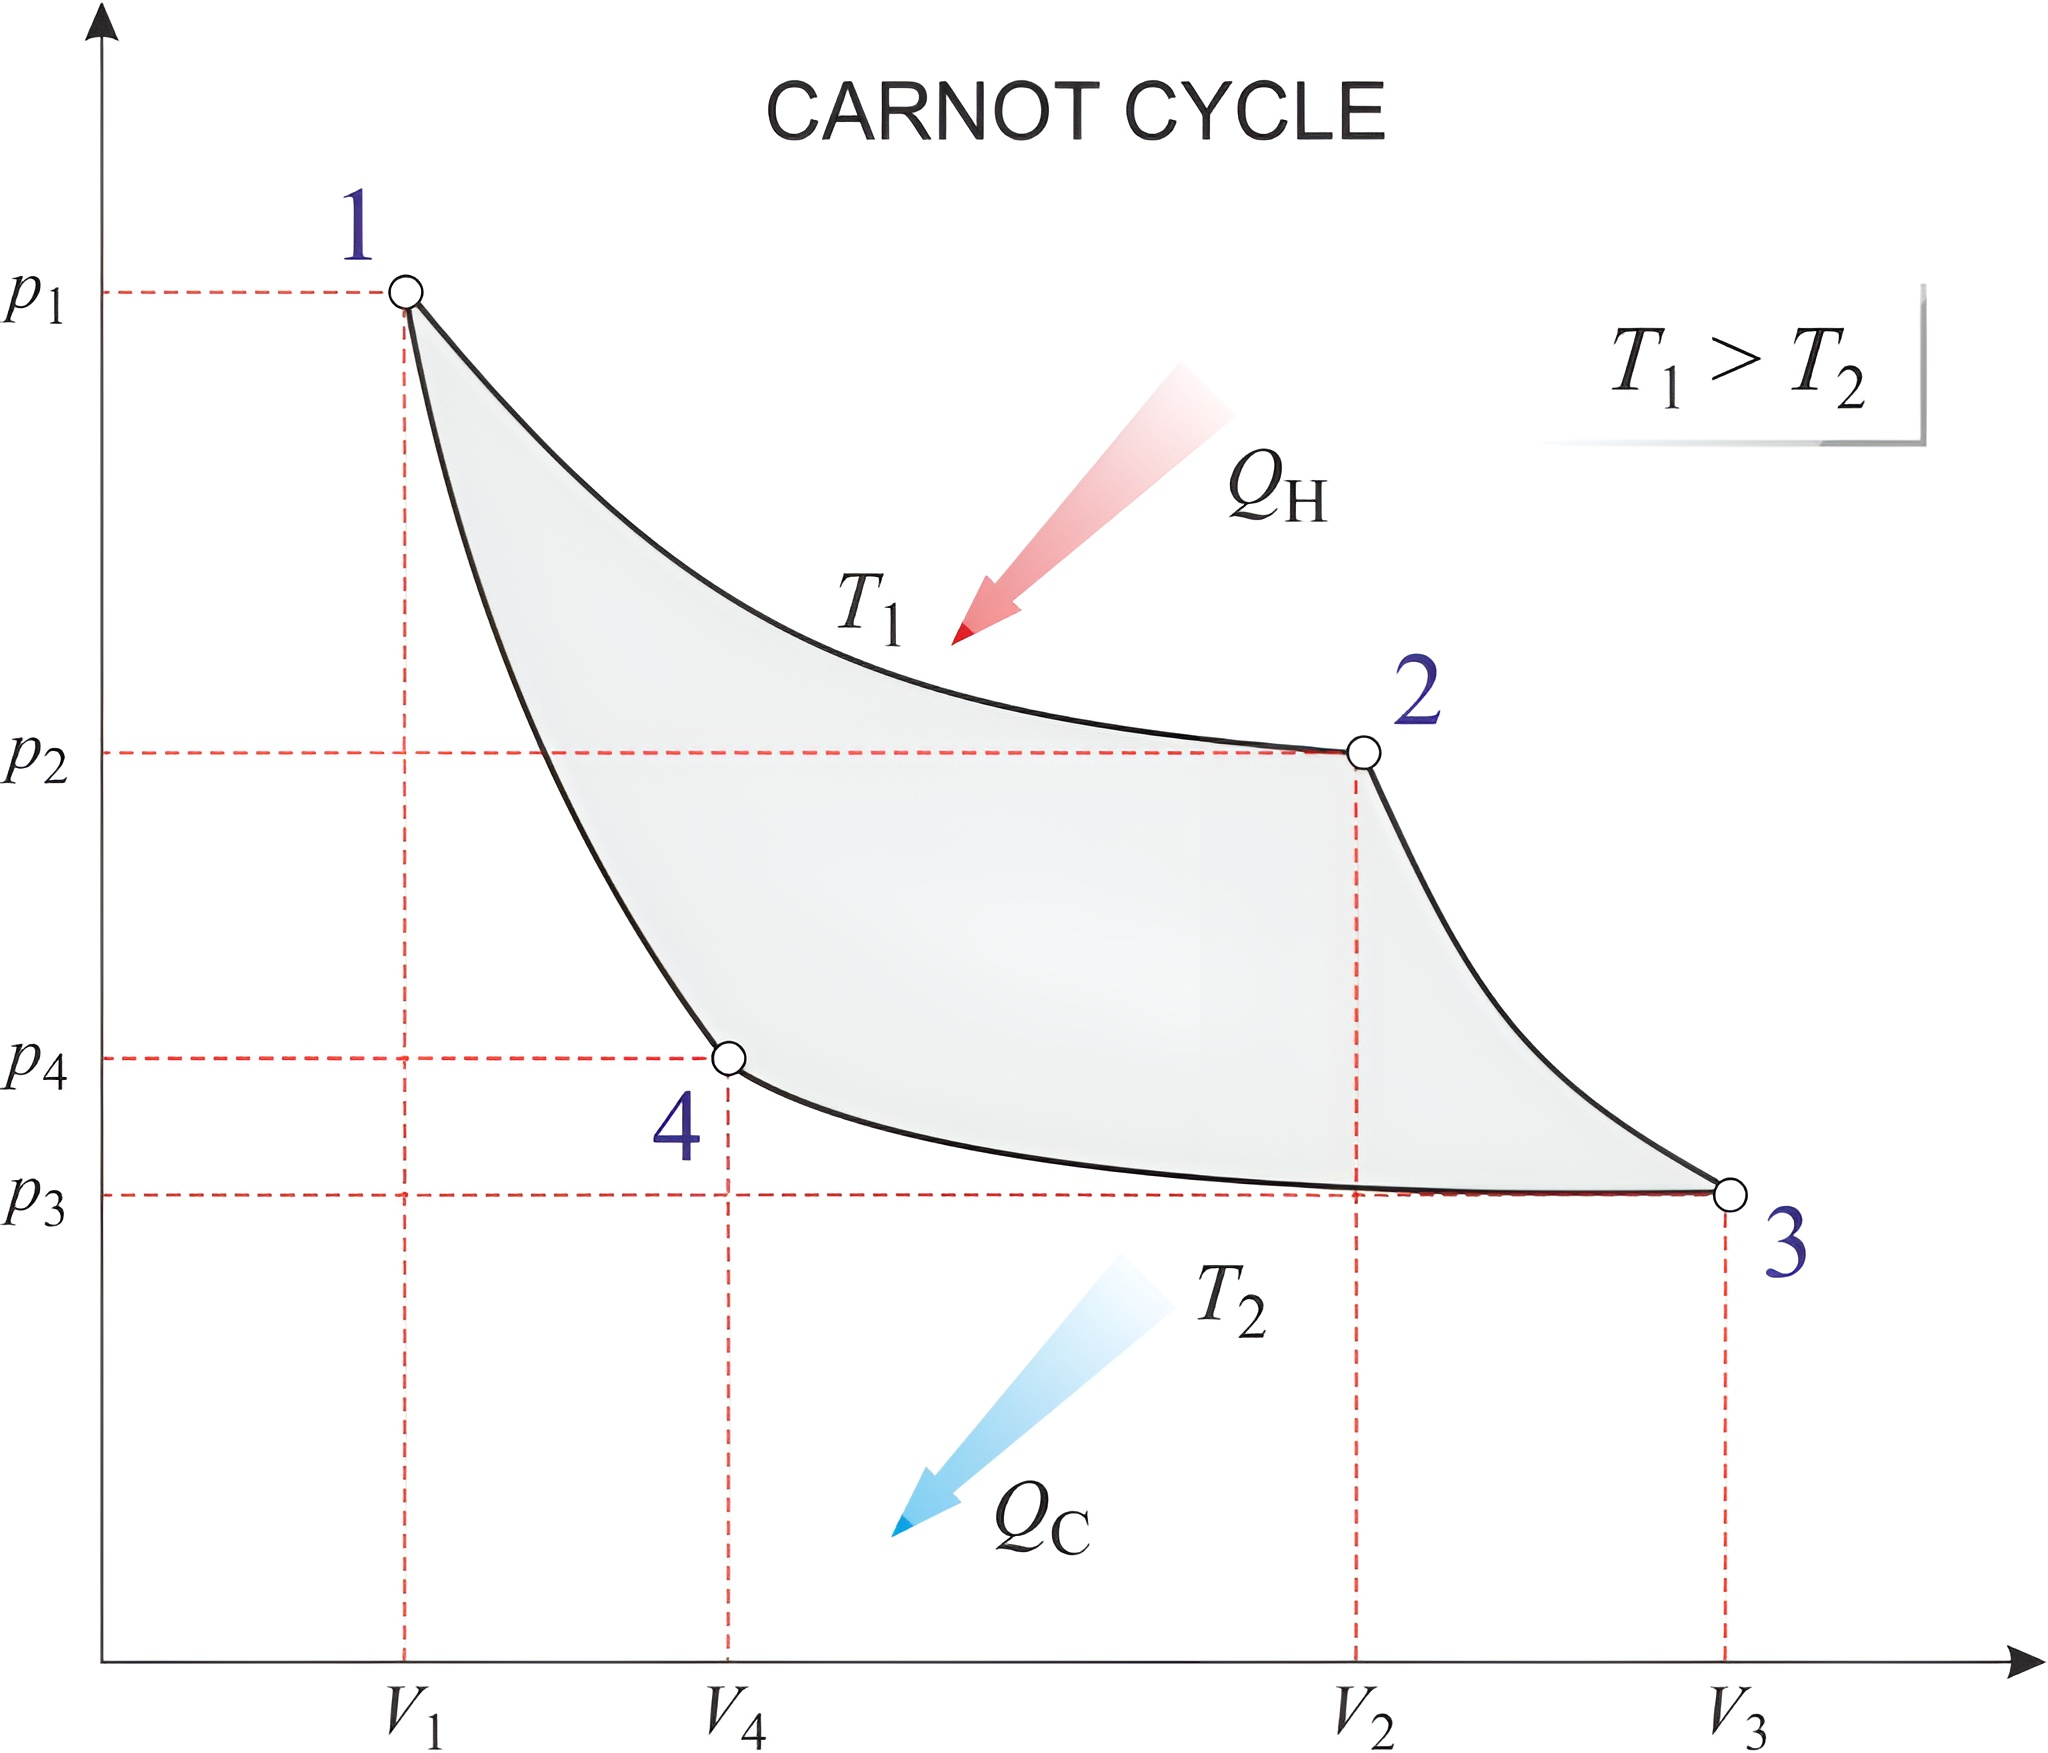
\includegraphics[width=0.4\textwidth]{Graphics/Carnot_Cycle.png}  % Adjust the width of the image
    \caption{PV-Diagram of Carnot Cycle: Heat is extracted from the hot reservoir, some of it is converted into work and some passed onto the cold reservoir. \cite{Eni}}
    \label{fig:Carnot_Cycle}
\end{figure}

Note that any of the steps outlined below can be the starting point: \cite{DINCER2018125}


% refer to figure
\begin{enumerate}
    \item \textbf{Isothermal expansion (1-2)}: Heat is absorbed from the hot reservoir at constant temperature, until equilibrium is reach. In the process, the volume grows.
    \item \textbf{Adiabatic compression (2-3)}: Gas stays in the same reservoir without heat transfer. Permitting it to expand the volume, the gas will deliver work in an adiabatic expansion.
    \item \textbf{Isothermal compression (3-4)}: Heat is transferred to the cold reservoir at constant temperature, until equilibrium is reached. The volume shrinks as a result.
    \item \textbf{Adiabatic expansion (4-1)}: Gas stays in the same reservoir without heat transfer. Work is done on the gas, transforming the gas into its original thermodynamic state. 
\end{enumerate}

For an ideal gas Carnot Cycle, the efficiency is simplified: \cite{BARBIR201317}

\begin{equation}
\label{eq:Carnot_Efficiency}
    \mathit{\eta = 1 - \frac{T_c}{T_h}}
\end{equation}

Using the same hot and cold reservoirs, work can be produced over a variety of processes. That being said, the efficiency of any other cycle has to be lower than the one calculated in Equation \ref{eq:Carnot_Efficiency}.

\subsection{Hypothesis}
\label{Hypothesis}

The first part of the lab session centers around verifying that the gas contained in the tube can be considered ideal. Although air is composed of multiple types of molecules, the majority of them could be considered to act similarly. Air can definitely not be considered an ideal gas, especially due to interactions between the molecules, but its macroscopic behaviour under the temperature and pressure conditions involved should somewhat match that exhibited by an ideal gas.

In the second part, the apparatus will be tested on a specific cycle. Using these results, one can calculate the heat engine's efficiency and compare it to the one theoretically obtained by a Carnot cycle. The heat engine's efficiency is expected to be far lower than the Carnot efficiency, mainly due to the simplicity of the setup. Additionally, leaks and frictional forces could affect the results, leading to higher deviations.
\newpage
\section{Materials \& Methods}

The session is divided into two parts, one checking if the air inside the apparatus can be considered ideal and one simulating a thermodynamic cycle. However, the main setup will be similar, with the equipment taken from the PASCO product TD-8572A, found at \cite{PASCO2024CavMan}.

\begin{wrapfigure}{r}{0.35\textwidth}  % 'r' for right, and width of 0.4 of the text width
    \centering
    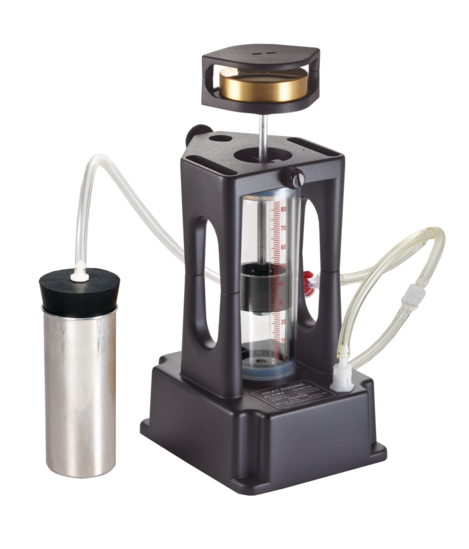
\includegraphics[width=0.35\textwidth]{Graphics/Apparatus.png}  % Adjust the width of the image
    \caption{Main apparatus of the heat engine, consisting of a thermal can connected to the Gas Law Apparatus. \cite{PASCO2024CavMan}}
    \label{fig:Apparatus}
\end{wrapfigure}

The main compartments of the heat engine were a metal thermal can and the Gas Law Apparatus. In the latter, a piston of radius $\mathit{r_p = (1.625 \pm 0.005)cm}$ could be found inside a glass cylinder with readings outside. The piston's movement could be controlled by either manually pushing the piston over a handle at the top, or screwing it at a fixed volume. If not fixed, the piston would smoothly increase the volume under higher pressures. Two ports for plastic tubes were available below the apparatus, both connected to the glass chamber. By connecting the metal can over plastic tubes to a Dual Pressure Sensor and one of these ports, air could only flow inside this system. The second port was also connected to the Dual Pressure Sensor to completely isolate the system. 

\begin{wrapfigure}{l}{0.4\textwidth}  % 'r' for right, and width of 0.4 of the text width
    \centering
    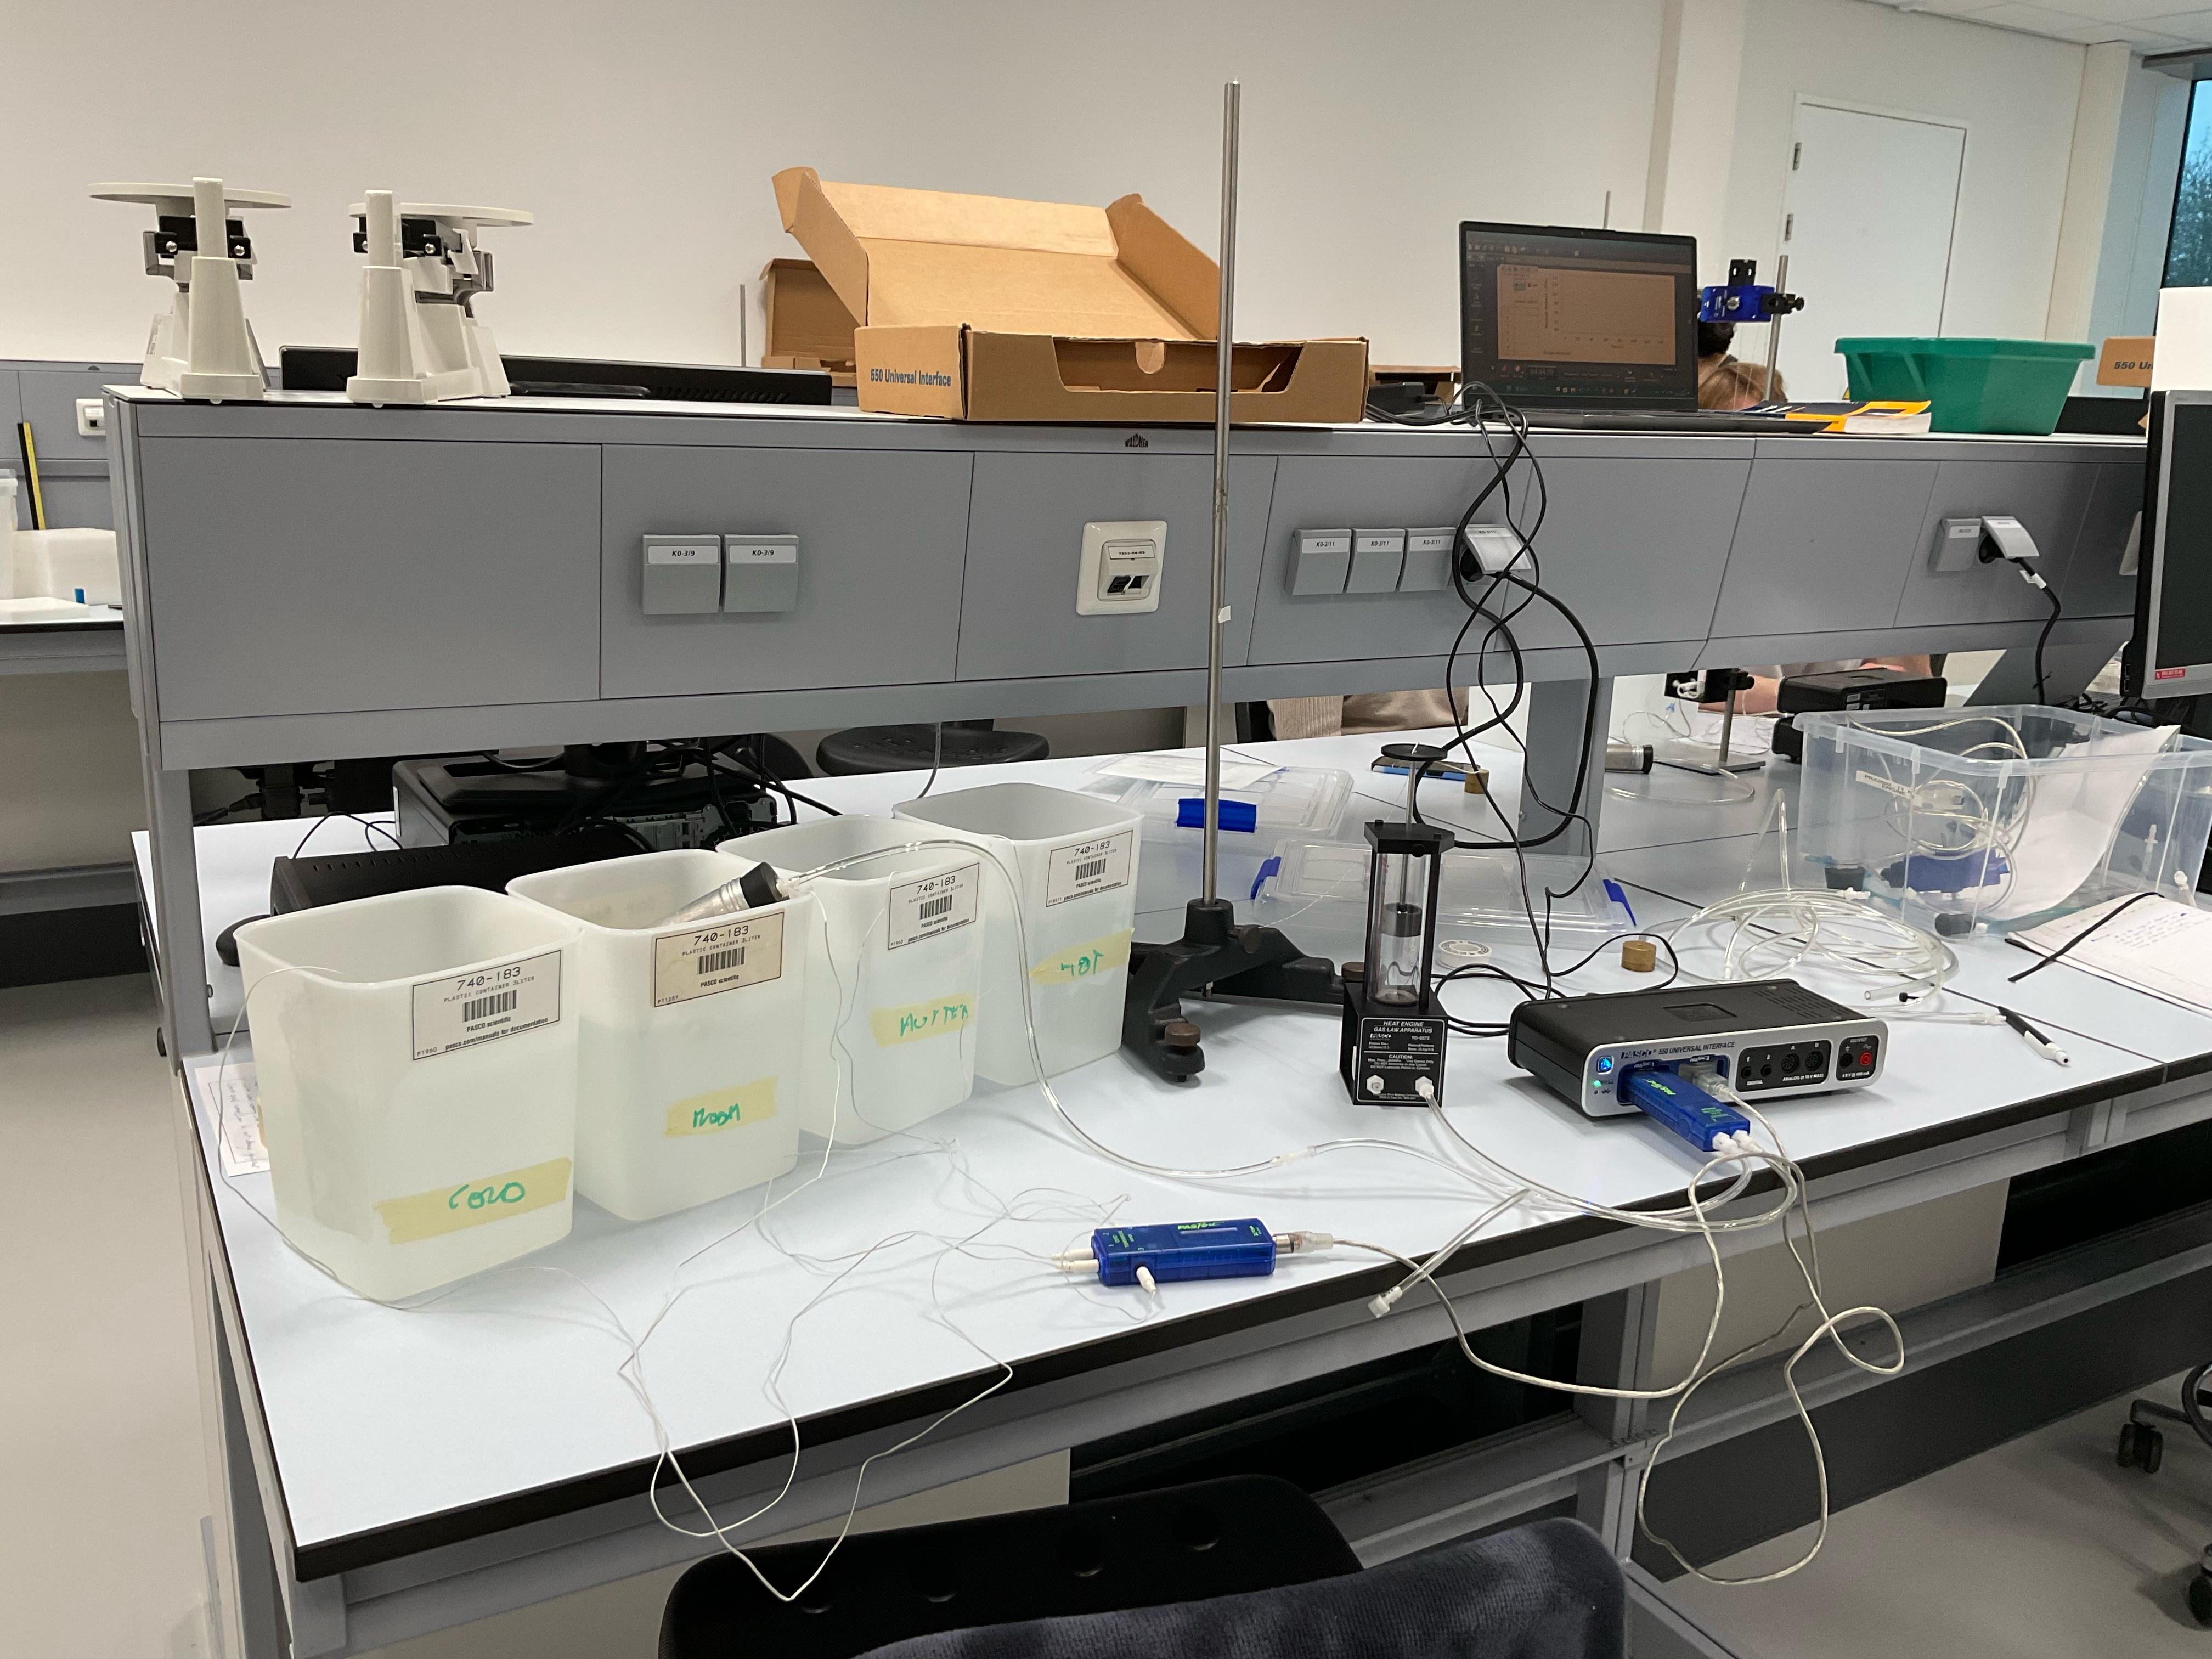
\includegraphics[width=0.35\textwidth]{Graphics/Ideal_Gas_Setup.jpeg}  % Adjust the width of the image
    \caption{Setup for ideal Gas Law Experiment. For comparison: The height of the metal rod inside the base is approx. 0.5m.}
    \label{fig:Ideal_Setup}
\end{wrapfigure}

For both experiments, the Dual Pressure Sensor and a Quad Temperature Sensor were connected over a PASCO Interface to PASCO Capstone, where the measurements could be quickly compiled. According to the producer, the device can read temperatures of all baths with an accuracy of approx. $\mathit{\pm 0.5 K}$.


\subsection{Evaluation Ideal Gas}
\label{Evaluation Ideal Gas}

To visualize the gas' ideality (i.e. how close its behaviour is to that of an ideal gas), the idea was to check one of the laws outlined in Section \ref{Ideal Gas Law}. It was decided to keep the volume constant and change the system's temperature, measuring the resultant pressure. An ideal gas would obey Gay-Lussac's Law (Equation \ref{eq:Gay-Lussac's Law}) and portray a positive linear correlation between pressure and temperature. As such, the piston was fixed over the screw.

Four thermal baths were prepared, each at vastly deviating temperatures. Fast Response Temperature Probes connected to the temperature sensor were placed in each container, with the readings documented in PASCO Capstone. 

Before conducting the measurements, a difficulty had to be addressed. At higher temperatures, the apparatus seemed to leak, meaning that over time the moles of gas $\mathit{n}$ would increase or decrease to adapt the system's pressure to its surroundings. Before each data logging, the apparatus was thus reset by unplugging the plastic tubes and placing the metal can inside a bath close to room temperature. The system was then isolated again, such that the can could be moved to the next reservoir. 

The data collected was used to plot a graph supposedly portraying the linear correlation between pressure $\mathit{P}$ and temperature $\mathit{T}$. 

\subsection{Simulating a Thermodynamic Cycle}
\label{Therm Cycle}

\begin{wrapfigure}{l}{0.4\textwidth}  % 'r' for right, and width of 0.4 of the text width
    \centering
    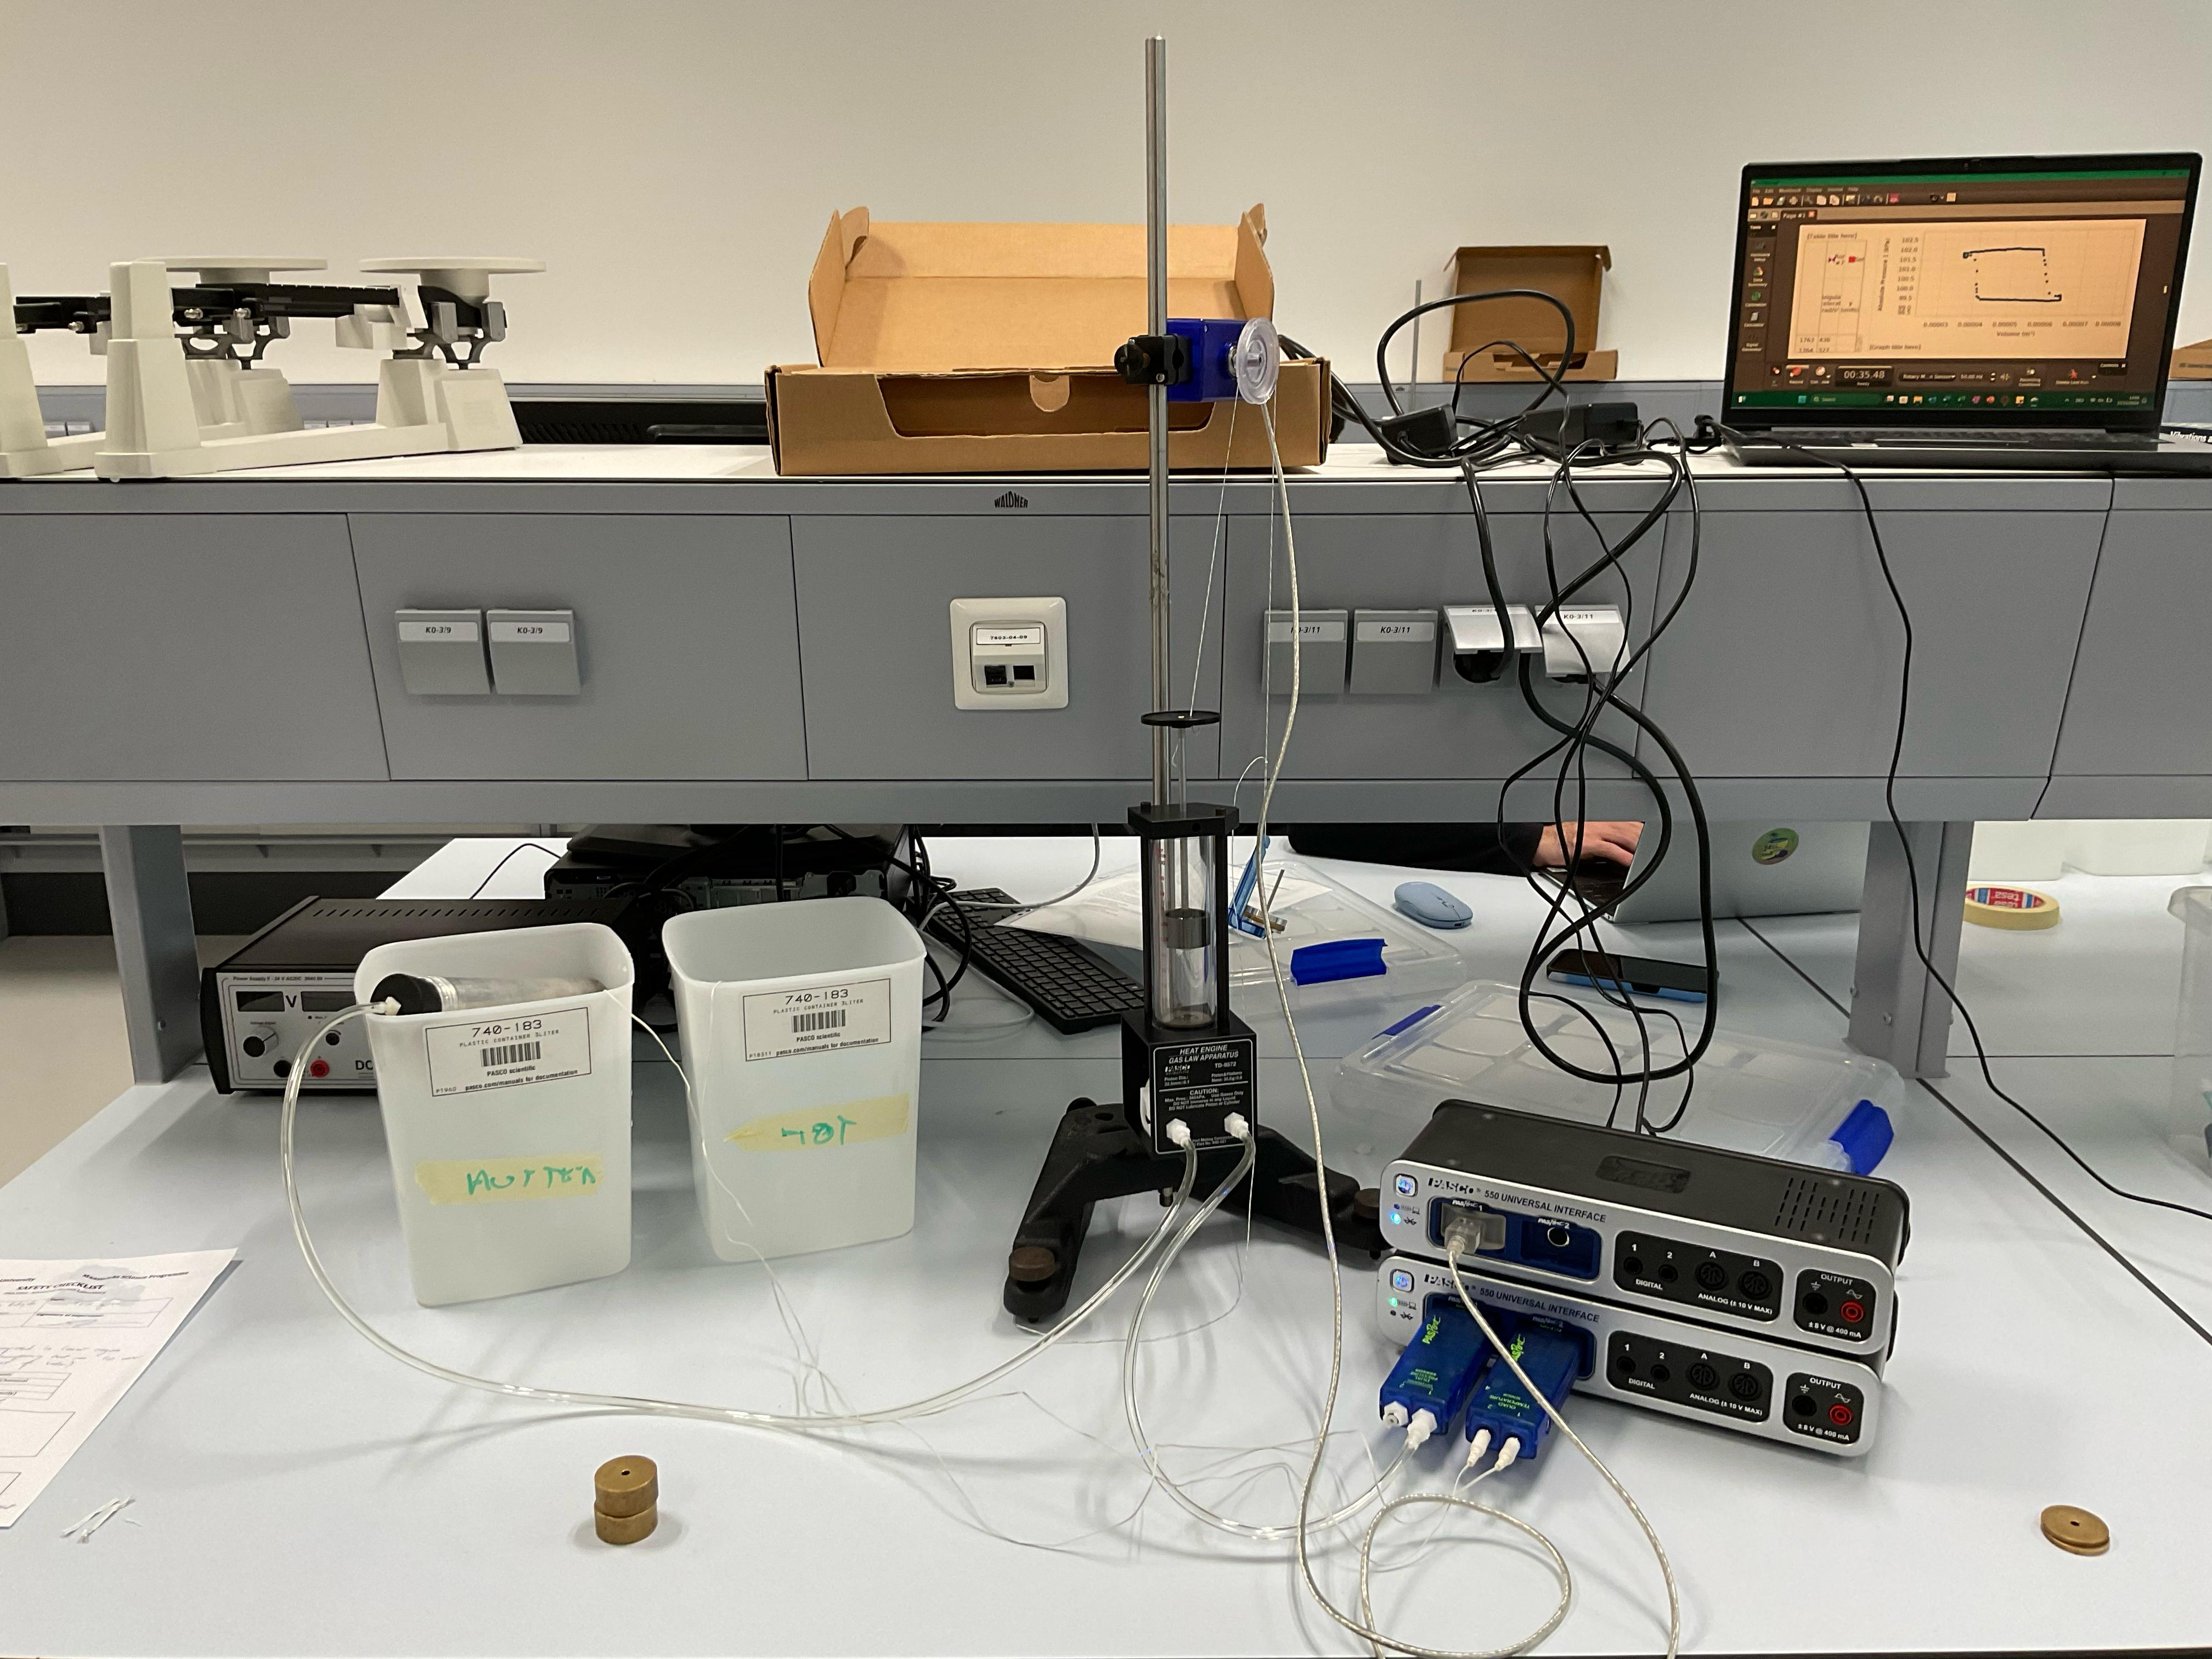
\includegraphics[width=0.35\textwidth]{Graphics/Cycle_Setup.jpeg}  % Adjust the width of the image
    \caption{Setup for Thermodynamic Cycle.}
    \label{fig:Cycle_Setup}
\end{wrapfigure}

The second part of the lab session considered the apparatus undergoing a thermodynamic cycle, closely resembling the Ericsson cycle. Two heat baths representing the hot and cold reservoirs were prepared, at temperatures vastly deviating from one another such that changes during thermodynamic processes could occur quickly. The temperatures were again measured through probes. 

The cycle consisted of four distinct processes, for which the setup had to be slightly altered. To begin with, the screw fixing the piston was removed in order to allow volumetric changes, which were assessed by a Rotary Motion Sensor. 

\begin{wrapfigure}{r}{0.35\textwidth}  % 'r' for right, and width of 0.4 of the text width
    \centering
    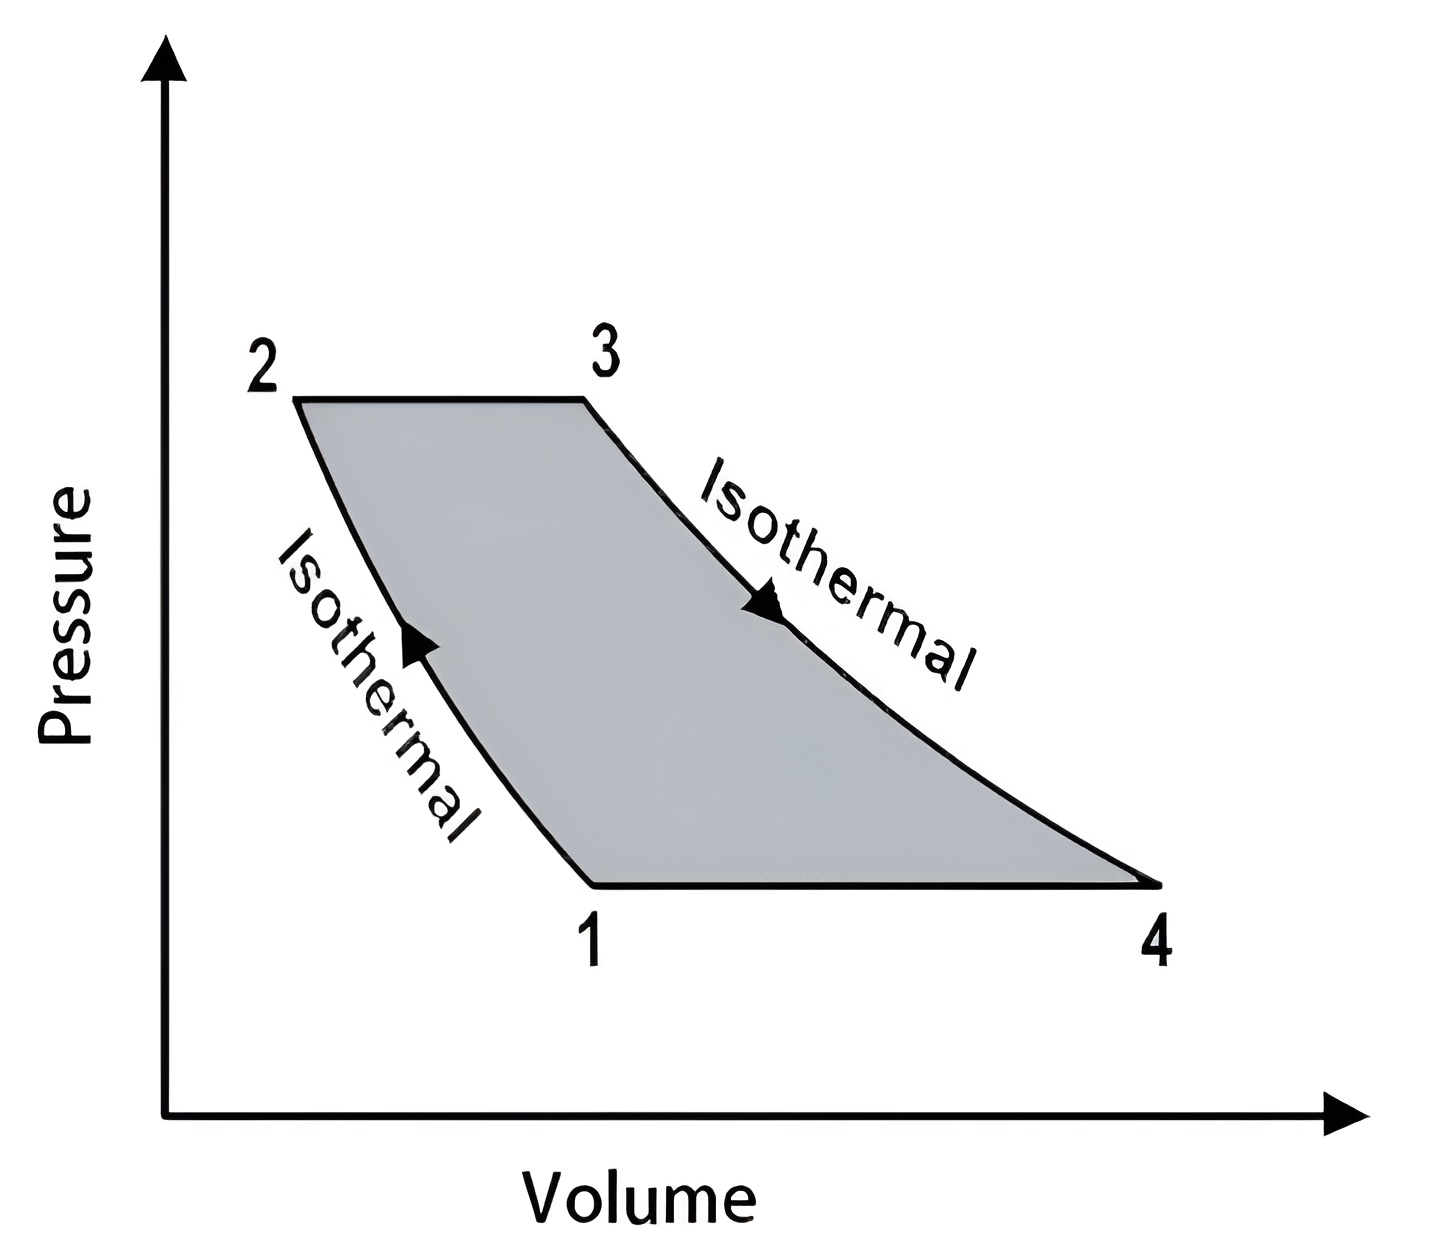
\includegraphics[width=0.45\textwidth]{Graphics/Ericsson_Cycle.png}  % Adjust the width of the image
    \caption{PV-Diagram of Ericsson Cycle: Two isothermal, two isobaric processes.}
    \label{fig:Ericsson Cycle}
\end{wrapfigure}

To counteract the weight of the piston pulling it down, equal masses were attached to it over a pulley. One could thus move the piston to a known initial position $\mathit{y_0}$ and leave it unperturbed. Although its position was originally set at $\mathit{y_0} = 0.05 m$, it was later realized that initial position had been altered during the several cycles in both directions by about $\mathit{\varepsilon_{y_0}= 0.003m}$. $\mathit{y_0 = (0.05 \pm 0.003) m}$ will be used following onwards. 

Since the volume of the plastic pipes and the metal can were not appraised by this group, the corresponding values will be taken from the student group surrounding Ana Tejero: $\mathit{V_{can} = 191.25 cm^3}$ and $\mathit{V_{pipes} = 13.09 cm^3}$. The total volume of the system can thus be calculated by:

\begin{equation}
\label{eq:Volume}
    \mathit{V = V_{can} + V_{pipes} + \pi r_p^2 (y_0 + y)}
\end{equation}

Here, $\mathit{y}$ is the displacement from initial position as measured by the Rotary Motion Sensor. From the formula, it can be seen that the error on the volume becomes $\mathit{\varepsilon_V = \pi r_P^2 \varepsilon_{y_0} \approx 2.489 \cdot 10^{-6} cm^3}$. Unfortunately, no uncertainties on the other volume values are known.

The setup was first acclimatized to room temperature. After plugging the open plastic tube into the apparatus and thus isolating the system, the can was placed in the cold reservoir and a PV-diagram was created. 

\textbf{Step I} will be thought of as displaying an isothermal compression, where a mass with $\mathit{m = 200g}$ was placed on top of the piston. However, later contemplations found in Section \ref{Thermodynamic Cycle Discussion} will contradict this approximation.

Next, in the isobaric expansion of \textbf{step II}, the metal can was moved to the hot reservoir and left there until the volume stopped increasing, meaning that equilibrium had been reached. 

After removing the mass (\textbf{step III}) and initiating an isothermal compression, the thermal can was inserted into the cold reservoir (\textbf{step IV}), a process of isobaric compression. 

The measurement was stopped when the PV-curve reached its original position.

Even though the process was repeated several times, only data from the first cycle will be analyzed, due to the error in the initial position being the lowest.

\subsubsection{Determining the Efficiency}
\label{Determining the Efficiency}

Over the temperatures of the cold and hot reservoirs measured at the beginning of each cycle, one could apply Equation \ref{eq:Carnot_Efficiency} to find the Carnot efficiency. Here, $\mathit{T_h = T_2 = T_3}$ and $\mathit{T_c = T_1 = T_4}$

Using Equation \ref{eq:Efficiency}, it is possible to calculate the engine's actual efficiency. The simplest method is to assess the area enclosed by the graphs in the PV-diagram, yielding the total work $\mathit{W}$ done per cycle. Additionally, by analyzing the type of thermodynamic process during each step, one can identify those where heat $\mathit{Q_h}$ was added to the system. 

In the described process, this would refer to the isobaric expansion in step II and the isothermal expansion in step III. Step III occurs at constant temperature, meaning that the internal energy is not affected: $\mathit{\Delta U_{III} = 0}$. From the Ideal Gas Law, it is found that $\mathit{P_3 V_3 = P_4 V_4 = const}$ during the process. The First Law of Thermodynamics can therefore be simplified:

\begin{equation}
\label{eq:Q_III}
    \mathit{Q_{III} = W_{III} = \int_{V_3}^{V_4} PdV = \int_{V_3}^{V_4} \frac{nRT}{V}dV = P_4 V_4 \ln{\frac{V_4}{V_3}}}
\end{equation}

At the end, $\mathit{P_4}$ and $\mathit{V_4}$ are chosen for convenience. 

Step II happens at constant pressure. 
The system the experiment centers around contains air, for which the composition is dominated by diatomic gases. Due to the degrees of freedom, the values for the specific heat capacities are given by $\mathit{C_V = \frac{5}{2}R}$ and $\mathit{C_P = \frac{7}{2}R}$. Equation \ref{eq:C_P} can be applied therefore:

\begin{equation}
\label{eq:Q_II}
    \mathit{Q_{II} = \frac{7}{2}nR \Delta T = \frac{7}{2} \frac{P_3 V_3}{T_h} (T_h-T_c) = \frac{7}{2} \frac{P_4 V_4}{T_h} (T_h-T_c)}
\end{equation}

The total heat absorbed is a combination of these two processes: $\mathit{Q_h = Q_{II} + Q_{III}}$.
The efficiency can be calculated from work $\mathit{W}$ and $\mathit{Q_h}$ alone.
\newpage
\section{Results \& Analysis}

\subsection{Ideal Gas: Results}
\label{Ideal Gas Results}

When inserting the metal can into the thermal baths and starting a measurement, the pressure either abruptly spiked or shrank. The pressure graph then met its extreme value and due to leakage, it quickly rebound to pressure at room temperature, as seen in Figure \ref{fig:P-time graph comp (cold vs hot)}. The extreme value is chosen as the desired value for the given temperature. 

\begin{figure}[H]
    \centering
    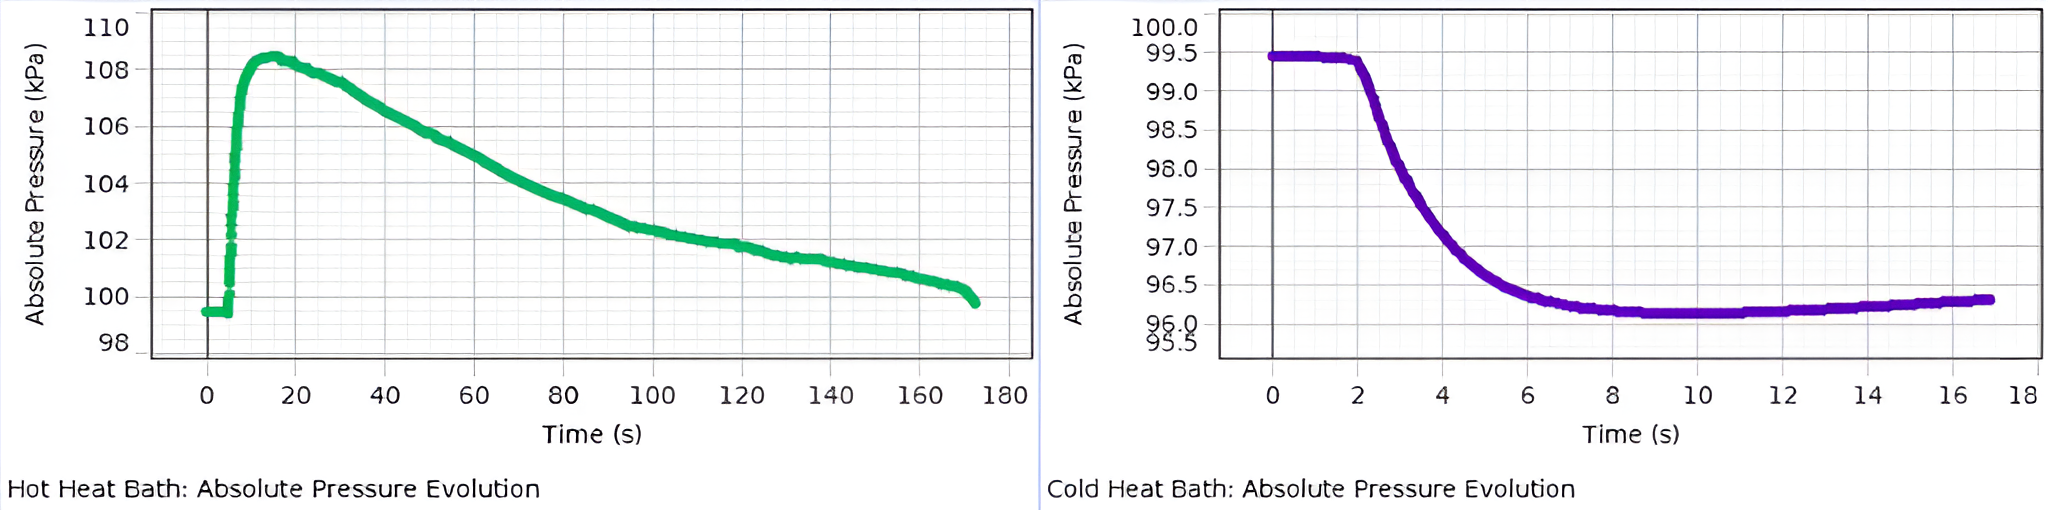
\includegraphics[width=1\linewidth]{Graphics/P_Evolution.png}
    \caption{Evolution of Pressure inside the system over time. Left: Pressure increases after inserting the can into a hot reservoir, the pressure used corresponds to the maximum. Right: Pressure decreases after inserting the can into a cold reservoir, the pressure used corresponds to the minimum.}
    \label{fig:P-time graph comp (cold vs hot)}
\end{figure}

Some fluctuations occurred at the begin of the data logging process, which affected the temperature inside the system. The temperature values will therefore possess additional uncertainties due to lack of knowledge about the precise value. Compiling all runs:

\begin{table}[H] 
    \setlength{\tabcolsep}{8pt} % Adjust column separation for clarity
    \renewcommand{\arraystretch}{1.3} % Adjust row height for better spacing
    \centering
    \small % Smaller font size
    \begin{tabular}{|c >{\centering\arraybackslash}p{4cm}|} % Set specific width for all columns
    \hline
     \textbf{Pressure [kPa]} &  \textbf{Temperature [\degree C]} \\ \hline \hline
    95.135 & $9.978 \pm 0.516$ \\ \hline
    100.808 & $29.125 \pm 0.510$ \\ \hline
    104.218 &  $42.250 \pm 0.515$ \\ \hline
    108.500 & $63.989 \pm 0.550$ \\ \hline
    \end{tabular}
    \caption{Checking Gay-Lussac's Law: Temperature against Pressure measurements from the various heat baths.}
    \label{tab:Ideal_Gas_Law}
\end{table}

For air to be an ideal gas, it must obey Gay-Lussac's Law, which declares a linear correlation between temperature and pressure when other variables are held constant. The data from Table \ref{tab:Ideal_Gas_Law} are therefore plotted, fitting a linear function of type $\mathit{Ax + B}$. The result is shown in Figure \ref{fig:P-time}.


\begin{figure}[H]
    \centering
    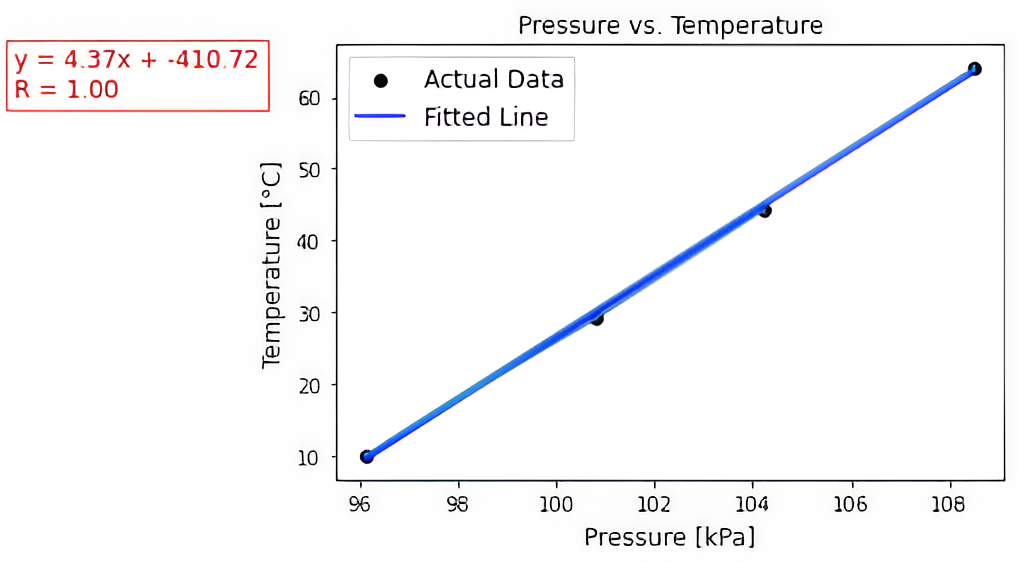
\includegraphics[width=0.5\textwidth]{Graphics/Ideal_Gas_plot.png}
    \caption{Checking Gay-Lussac's Law: Graph plotting Pressure vs Temperature. A linear function is fitted to the graph, with a correlation coefficient of $\mathit{R=1}$.}
    \label{fig:P-time}
\end{figure}

The linear correlation is verified, with a correlation coefficient of $\mathit{R = 1.00}$. One can therefore proceed with the ensuing experiment.

\subsection{Thermodynamic Cycle: Results}
\label{Therm Cycle Results}

The cycle of the first data run was chosen for analysis. A PV-diagram of the collected data is depicted in Figure \ref{fig:Cycle_Exp}. Some points had to be deleted, as Capstone could not properly connect certain points. This had been due to the frequencies of the Rotary Motion Sensor and Pressure Sensor being different, where 5 pressure values were found for every 2 position values. 

Nonetheless, the total work could properly estimated as $\mathit{W = 0.0618 J}$.

\begin{figure}[H]
    \centering
    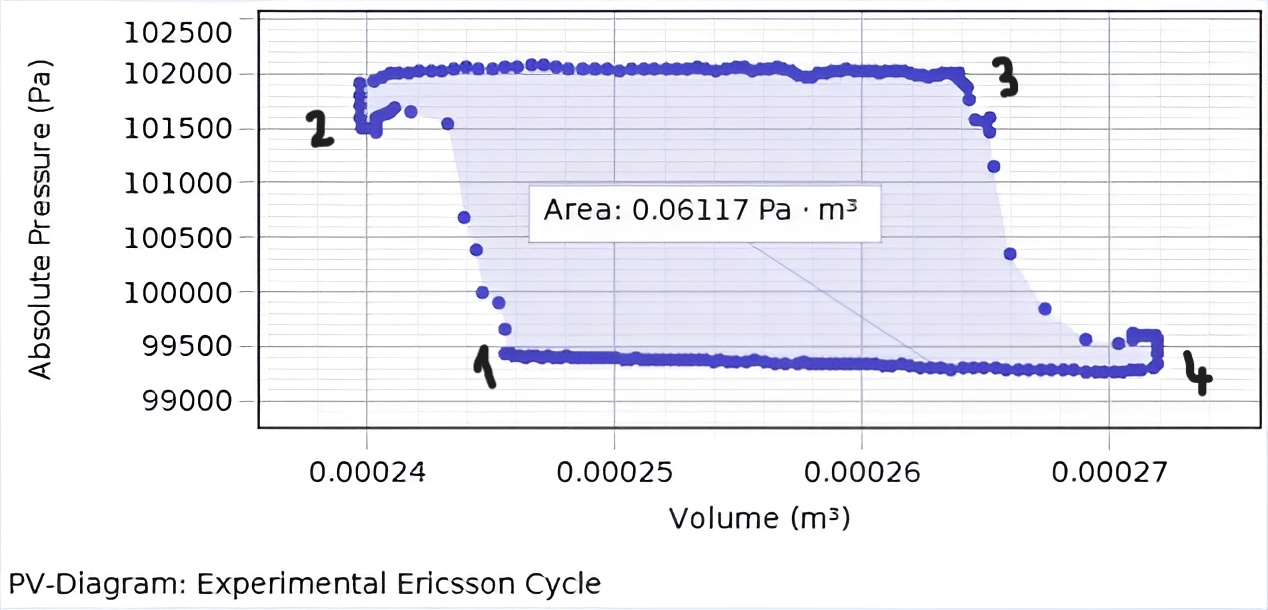
\includegraphics[width=0.6\linewidth]{Graphics/PV-Diagram_Ericsson.png}
    \caption{PV-Diagram of the simulated quasi-Ericsson Cycle. The process is initiated at equilibrium point 1, and cycles over 4 thermodynamic processes back to its original position. The area inside the graph represents the work per cycle.}
    \label{fig:Cycle_Exp}
\end{figure}

Temperatures of the baths were given by $\mathit{T_1 = T_2 = T_c = (284.285 \pm 0.500) K}$ for the cold reservoir and $\mathit{T_4 = T_3 = T_h = (324.758 \pm 0.500) K} $ for the hot one. The temperatures stayed constant over the isothermal paths. Furthermore, equilibrium point 1 corresponds to the initial position, with a volume of $\mathit{V_1 = \pi r_p^2 y_0 + V_{can} + V_{pipes} \approx (2.458 \pm 0.025) \cdot 10^{-4} m^3}$. 

% pressure errors by looking at the deviations along the cosntant line

The cycle consisted of two isobaric processes. To assess the corresponding pressures, an average of the values between equilibrium points 2 and 3 as well as 4 and 1 was determined, with the approximate deviations from the constant line representing the uncertainties. For further calculation $\mathit{P_2 = P_3 = (102011 \pm 25) Pa}$ and $\mathit{P_1 = P_4 = (99290 \pm 75) Pa}$ are utilized.

During process IV, between points 4 and 1, the ratio $\mathit{\frac{V}{T}}$ stayed constant. As a result, $\mathit{V_4}$ can also be expressed as:

\begin{equation}
\label{eq:V_4}
    \mathit{V_4 = V_1 \frac{T_h}{T_c}}
\end{equation}

Furthermore, the isothermal process III between points 3 and 4 implied that for that duration, $\mathit{PV = const}$. $\mathit{V_3}$ can thus be written as:

\begin{equation}
\label{eq:V_3}
    \mathit{V_3 = V_4 \frac{P_4}{P_3}}
\end{equation}

These relation can be implemented when calculating the heat absorbed during the cycle. For process II, Equation \ref{eq:Q_II} will be used for the calculations:
% error on pressure negligible

\begin{equation}
\label{eq:V_T const}
    \mathit{Q_{II} = \frac{7}{2} \frac{P_4 V_4}{T_h}(T_h - T_c) \approx (11.8545 \pm 0.3186) J}
\end{equation}

The errors included above are governed by the error propagation of all variables included in the formula. Noting that the error in pressure can be neglected, the relative error is given by Equation \ref{eq:Q_II_Error}:

\begin{equation}
    \label{eq:Q_II_Error}
    \mathit{\frac{\Delta Q_{II}}{Q_{II}} = \sqrt{(\frac{\varepsilon_{V_4}}{V_4})^2 + (\frac{\varepsilon_{T_h}}{T_h})^2 + (\frac{\varepsilon_{T_h} + \varepsilon_{T_c}}{T_h -T_c})^2} \approx 0.0269}
\end{equation} 

A similar procedure can be conducted for the isobaric process III:

\begin{equation}
\label{eq:T const}
    \mathit{Q_{III} = P_4 V_4 \ln{\frac{V_4}{V_3}} \approx (0.7514 \pm 0.5033) J}
\end{equation}

Here, the error is also gained from analyzing the error propagation. Noting that the error for a function of type $\mathit{\ln{x}}$ is $\mathit{\Delta \ln{x} \approx \frac{\Delta x}{x}}$, and $\mathit{\ln{\frac{V_4}{V_3}} = \ln{V_4} - \ln{V_3}}$: 

\begin{equation}
    \label{eq:Q_III_Error}
    \mathit{\frac{\Delta Q_{III}}{Q_{III}} = \sqrt{(\frac{\varepsilon_{V_4}}{V_4})^2 + (\frac{\frac{\varepsilon_{V_4}}{V_4} + \frac{\varepsilon_{V_3}}{V_3}}{lnV_4-lnV_3})^2} \approx 0.6698}
\end{equation}

The high uncertainty can be traced back to the small difference between the volumes, causing the logarithmic function to be sensitive to small changes.

Equation \ref{eq:Q_tot} portrays the total heat absorbed in the process.

\begin{equation}
\label{eq:Q_tot}
    \mathit{Q_{h} = Q_{II} + Q_{III} = (12.6059 \pm 0.8219) J}
\end{equation}

Finally, one can insert the values for work $\mathit{W}$ and heat $\mathit{Q_h}$ to find the heat engine's actual efficiency:

\begin{equation}
\label{eq:Exp_Efficiency}
    \mathit{\nu = \frac{W}{Q_h} \approx 0.00485 \pm 0.00032}
\end{equation}

If the cycle were that of an ideal Carnot Cycle, the efficiency would instead be the one calculated below:

\begin{equation}
\label{eq:Exp_Carnot_Efficiency}
    \mathit{\eta =  1-\frac{T_c}{T_h} \approx 0.12186 \pm 0.00028}
\end{equation}

One can see that the maximum efficiency of the engine is clearly not reached by the conducted cycle. In fact, the engine only works at approx. $\mathit{3.98 \%}$ of its ideal thermodynamical efficiency.
\newpage
\section{Discussion}
\label{Discussion}

During the experiment, the gas inside an apparatus consisting of a metal can connected to a container with a movable piston was checked for its ideality. The goal was met by varying the temperature $\mathit{T}$ at constant volume $\mathit{V}$ and observing the changes in pressure $\mathit{P}$. Afterwards, the system underwent an Ericsson cycle, where the efficiency of the heat engine was calculated and compared to the ideal one found during a Carnot cycle. Section \ref{Theory} contains a few predictions towards the experiment's outcome.

\subsection{Ideal Gas Law Experiment: Discussion}
\label{Ideal Gas Discussion}

When inserting the can into the heat baths, one could observe a sudden spike in pressure, followed by a steady decline towards room temperature levels. One can attribute the decline to the leakage of molecules. Especially more pronounced at higher temperatures and therefore pressures, the transition balances the pressures inside and outside.

From the collected data, it was possible to verify the positive linear correlation between pressure and temperature. The data points, when considering their uncertainties, all lie on a linear function fitted to it. Additionally, approximated to two decimal digits, the correlation coefficient was found to be $\mathit{R=1.00}$, visualizing the approximate ideal behaviour of the air contained in the system, in line with the prediction.

\subsection{Thermodynamic Cycle: Discussion}
\label{Thermodynamic Cycle Discussion}

The Ericsson cycle was based on two heat reservoirs at $\mathit{T_c} ) 284.29 K$ and $\mathit{T_h} ) 324.76 K$, with a net work of $\mathit{W=0.0618J}$. Exploiting constant quantities during specific processes allowed the determination the heat $\mathit{Q_h}$ absorbed in steps II and III. Summing them up yields $\mathit{Q_h = (12.6059 \pm 0.8219) J}$.

The heat engine's actual efficiency was thus found to be $\mathit{\nu = 0.00485 \pm 0.00032}$, with the ideal Carnot efficiency relative to the temperatures $\mathit{T_c}$ and $\mathit{T_h}$ being $\mathit{\eta 
= 0.12186 \pm 0.0028}$. The heat engine was therefore only able to achieve $\mathit{3.98 \%}$ of its maximum efficiency, which changes little when taking the uncertainties into account. 

Although somewhat expected, the heat engine appears to be highly impotent in producing apt work for the heat it absorbs. The simple materials could be an explanation, but specific precautions had been taken to prevent leaks. One fault can be found in the analysis. Paths I and III where described as being isothermal. Frankly, such kind of processes normally occur at slow speeds, so that the system does not experience changes in internal energy, keeping the temperature constant. However, altering the calculations for process III can do little to decrease the heat absorbed by the system, as process II contributes most to $\mathit{Q_{h}}$. 

\subsection{Changes to Experiment: Reducing the Uncertainties}
\label{Uncertainty Reduction}

Although the sample size was rather small, the results from the ideal gas experiment appear promising, in that they verify Gay-Lussac's law for the case of the air trapped in the metal can. That being said, the uncertainties on temperature have to be decreased for more precise measurements. For the coldest bath, the temperature is only known with 5 \% uncertainty. While the temperature probes themselves seem to work accurately, the Quad Temperature Sensor, with an accuracy of $\mathit{\pm 0.5K}$, could have considerable impact on the results. More precise temperature measurements therefore require a replacement.

For the Ericsson Cycle Experiment, numerous improvements can be made. For one, the determining the initial position $\mathit{y_0}$ of the piston inside the glass cylinder was done rather carelessly, with the reading guesstimated from the scale printed on the cylinder and the initial position changing throughout each cycle, with the lack of proper methods to evaluate these changes. Instead, one could have calibrated the Motion Sensor by completely compressing the piston and setting that position as 0. The reading would be accurate, and the subsequent cycles could be appropriately compared.

The previous suggestion already substantially decreases the uncertainty of measurement. Nonetheless, the error in $\mathit{Q_{III}}$ would still be considered significant. The degree thereof mostly originates from the logarithmic function. $\mathit{V_3}$ and $\mathit{V_4}$ deviate only little from one another, so small changes can have large impact. Between equilibrium points 3 and 4, the mass is removed from the system, meaning that implementing heavier masses imply bigger volume changes. However, the leaks would worsen as a result. Generally increasing the scale of the experiment would not alter the ratio $\mathit{\frac{V_4}{V_3}}$, the suggestion would thus be ineffective. As such, unless the problem with leakage in the system is fixed, more precise volumes remain the most constructive improvements. 

\subsection{Further experiments}
\label{Further experiments}

Generally, the ideal gas law experiment can be deemed successful, as the data fit almost perfectly to a linear function. One can thus apply other laws on the apparatus, such as Boyle's law or Charles' law. Under the conditions of the experiment conducted in this paper, the results should similarly be in agreement with theory. One could additionally implement higher temperatures, to observe when air stops acting ideal. The same idea could be implemented more easily by fixing the piston at smaller volumes. In such a scenario, pressure would increase more quickly under temperature changes. If the current apparatus is apt for such conditions remains to be seen, with its leaks being especially apparent at high pressure. 

Furthermore, as of now, only the thermal efficiency of the cycle has been discussed. However, one can also consider the actual usable work compared to the net work of the process. This would be seen in the displacement of the piston-mass complex, where a force equal to that of the mass' weight force would be acted over a certain distance. An interesting to observe how much of the net work is actually converted into the displacement work, meaning that one could find the mechanical efficiency. 


\newpage
\section{Conclusion}
\label{Conclusion}

The first experiment posed the question if the air contained in the apparatus can be considered ideal. By showing that pressure and temperature had a linear correlation with correlation coefficient $\mathit{R=1.00}$ when the other variables where held constant, Gay-Lussac's law was validated and the apparatus could be safely implemented for a thermodynamic cycle. 

The second experiment aimed at replicating Ericsson's cycle. From the data, the net work per cycle $\mathit{W}$ and the heat $\mathit{Q_h}$ absorbed were found, meaning that one could calculate the efficiency. The heat engine's actual efficiency was determined as $\mathit{\nu = 0.00485 \pm 0.00032}$, while the theoretical efficiency of a Carnot cycle would have been $\mathit{\eta = 0.12186 \pm 0.00028}$. The heat engine therefore worked at only $\mathit{3.98 \%}$ of its maximal thermal efficiency. 

Suggestions have been made to improve on the accuracy of the measurement. These contain finding a precise reference point for the volume inside the glass cylinder of the piston by calibrating the Rotary Motion Sensor, or observing more points for the ideal gas law experiment. Additionally, further experiments have been brought forth, namely that of calculating the mechanical efficiency or verifying the ideality of the system's air by checking other laws. 
\newpage
\printbibliography
\pagebreak
\end{document}
